\newpage
\section{Resultados}

\subsection{Resultados obtidos}

A figura \ref{f_img1} mostra um exemplo de figura.

\begin{figure}[H]
	\centering
	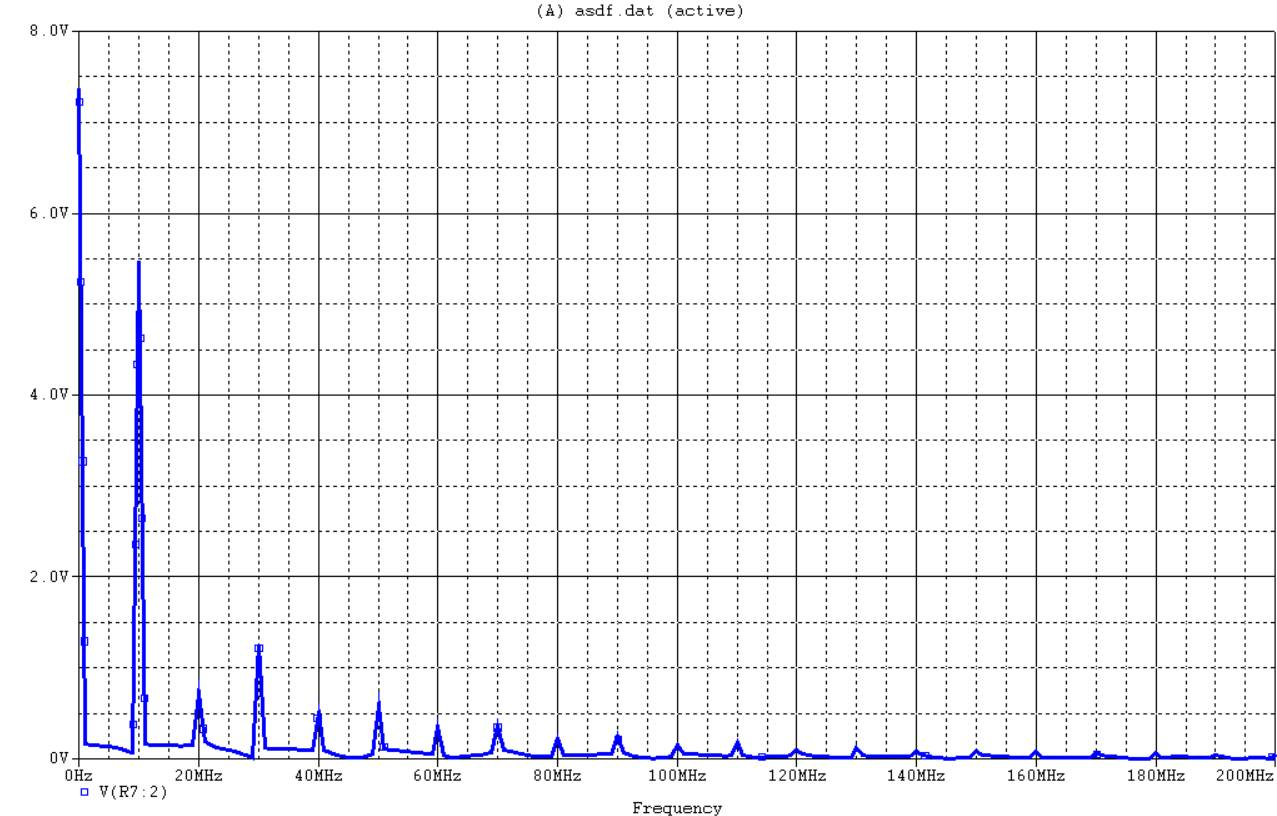
\includegraphics[scale=0.3]{img/img1.jpg}
	\caption{Exemplo de figura}
	\label{f_img1}
\end{figure}

A tabela \ref{t_tabela1} mostra um exemplo de tabela.

\begin{small}
	\begin{table}[H]
		\begin{center}
			\caption{Frequência de oscilação obtida variando-se a tensão de circuito}
			\begin{tabular}{l|l}
				\hline
				Tensão de & Frequência [MHz] \\
				entrada [V]&  \\
				\hline
				9.6 & 10.01071 \\
				\hline
				12.0 & 10.01088 \\
				\hline
				14.4 & 10.01119 \\
				\hline
			\end{tabular}
			\label{t_tabela1}
		\end{center}
	\end{table}
\end{small}

A equação \ref{e_equacao1} mostra um exemplo de equação.

\begin{equation}
y = \alpha.(x-x_0) + y_0
\label{e_equacao1}
\end{equation}